\chapter{Analiza wymagań}

\section{Wstęp}

%TODO Alternatywna wersja 

Wraz z rozwojem handlu konieczne stało się stowrznie miejsca w którym towary
będą składowane przed zakupem  przez klienta. W przypadku małych magazynów to
pracownicy są w stanie nim efektywnie zarządzać i efektywnie wyszukiwać towarów
znajdujących się w nim. Jednak co dzieje się w przypadku gdy magazyn jest
większy? Konieczne staje się stowrzenie systemu który umożliwi pracownikom
łatwiejsze i bardziej efektywne zarządzanie towarami znajdującymi się w
magazynie.

Głównym zadaniem systemu do zarządzania magazynem jest przechowywanie ilości
poszczególnych towarów. Możliwość przyjmowania dostaw jaki i również sprzedaży
towarów klientom. Powinien również przechowywać informacje o dostawcach,
towarach a także o klientach.

\subsection{Przeznaczenie systemu}

Głównym zadaniem systemu jest ułatwienie zarządzania magazynem pracownikom
magazynu, poprzez umożliwienie zarządzania klientami, dostawcami, towarami a
także zamównieniam sprzedaży jak i zakupu. System ten nie jest specjalizowany
pod konkrentną dziedzine handlu. Umożliwia on natomiast przechowywanie i
zarządznanie informacjami o towarach dowolnego typu. 

\subsection{Architektura systemu}

W obecnie towrzonych systemach spotyka się dwie podstawowe struktury:
architekturę klient-serwer oraz architekturę trójwarstwową.
W architekturze klient-serwer, która była szczególnie popularna w
latach dziewięćdziesiątych ubiegłego wieku, wyróżnia się
dwie warstwy: 
\begin{itemize}
 \item aplikację użytkownika (\emph{klient});
 \item system zarządzania bazą danych (\emph{serwer}).
\end{itemize}

Struktura ta sprawdza się dla prostych systemów, których zadaniem jest
zapisywanie, odczytywanie oraz aktualizacja danych. Problem
pojawia się jednak w przypadku, gdy dane muszą być przetwarzane w
nietrywialny sposób, przy uwzględnieniu dziedziny problemu (ang. \emph{domain
logic}) modelowanego zagadnienia. Realizacja obliczeń w warstwie klienta,
której głównym zadaniem jest prezentacja informacji użytkownikowi, może
znacząco wpływać na jego komfort pracy oraz powodować problemy związane z
duplikacją kodu źródłowego aplikacji.
Natomiast umieszczenie logiki aplikacji po stronie serwera bardzo często narzuca
przygotowanie programu w środowisku specyficznym dla danego systemu zarządzania
bazami danych. 

Problemy te zmusiły projektantów aplikacji do wydzielenia jeszcze jednego
poziomu, który jest odpowiedzialny za logikę operacji na danych. W
architekturze trójwarstwowej uwzględnione są następujące warstwy:
\begin{itemize}
 \item warstwa prezentacji;
 \item warstwa aplikacji;
 \item warstwa źródła danych.
\end{itemize}

%TODO Wstawić schemat prezentujący architekturę trójwarstwową.

W przypadku systemu do obsługi magazynu zdecydowano się wykorzystanie
architektóry trójwarstwowej.

\section{Aktorzy}

Aktorzy w zaprojektowanym systemie zostali podzieleni na dwie grupy: aktorów
osobowych oraz aktorów nieosobowych. Do aktorów osobowym można zaliczyć
wszystkich użytkowników projektowanego systemu, aktorami nieosobowymi są
natomiast wszystkie systemy zewnętrzne współpracujące z projektowanym systemem.
Poniższy diagram przedstawia hierarchie aktorów osobowych w systemie:

%TODO Wstawić diagram z aktorami osobowymi: administrator, magazynier,
% sprzedawca 
\begin{figure}[h]
    \begin{center}
    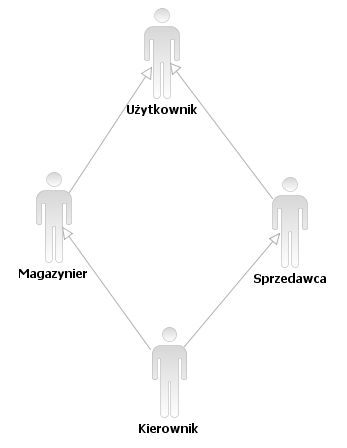
\includegraphics[scale=0.75]{../img/diagramDziedziczenia.png}
    \end{center}
    \label{fig:diagramDziedziczenia}
\end{figure}
\FloatBarrier



\section{Wymagania funkcjonalne}

Niniejsze rozdział zawiera zdefiniowane dla systemu wymagania funkcjonalne.

%\arrayrulecolor{line}
%\rowcolors{2}{cell}{white}

\begin{table}[ht]
	 \begin{center}
% 	    \rowcolors{1}{}{lightblue}
% TODO a wyszukiwanie
	    \begin{tabular}{| l | l | l | l | l |}%\toprule
	    	\hline
		    \textbf{Lp.} & \textbf{Nazwa}  & \textbf{Priorytet} & \textbf{Ryzyko} &
		    \textbf{Nazwa aktora} \\
		    \hline
		    1 & Zarządzanie użytkownikami & wysoki & niskie & administrator \\
		    1.1 & Dodawanie użytkowników & wysoki & niskie & adminstrator \\
		    1.2 & Edycja danych użytkowników & wysoki & niskie & adminstrator \\ 	
		    1.3 & Usuwanie danych użytkowników & wysoki &niskie & administrator \\
		    \hline
		    2 & Zarządzanie danymi towarów & wysoki & niskie & magazynier \\
		    2.1 & Dodawanie towaru & wysoki &  niskie & magazynier \\
		    2.2 & Edycja danych twarów & wysoki & niskie & magazynier \\
		    2.2.1 & Edycja opisu towarów & wysoki & niskie & magazynier \\
		    2.2.2 & Zmiana ilości towarów & wysoki & niskie & użytkownik \\
		    2.3 & Usuwanie danych towarów & wysoki & niskie & magazynier \\
		    \hline
		   	3 & Zarządzanie danymi klientów & wysoki & niskie & sprzedawca \\
		   	3.1 & Dodawanie klientów & wysoki & niski & sprzedawca \\
		   	3.2 & Edycja danych klientów & wysoki & niskie & sprzedawca \\
		   	3.3 & Usuwanie danych klientów & wysoki & niskie & sprzedawca \\
		   	\hline
		   	4 & Zarządzanie danymi dostawców & wysoki & niskie & magazynier \\
		   	4.1 & Dodawanie dostawców & wysoki & niskie & magazynier \\
		   	4.2 & Edycja danych dostawców & wysoki & niskie & magaziner \\
		   	4.3 & Usuwanie danych dostawców & wysoki & niskie & magazynier \\
		   	\hline
		   	5 & Zarządzanie zamowieniami sprzedaży & wysoki & niskie & sprzedawca \\
		   	5.1 & Tworzenie zamówień sprzedaży & wyskoki & niskie & sprzedawca \\
		   	5.2 & Edycja zamówień sprzedaży & wysoki & niskie & sprzedaca \\
		   	5.3 & Usuwanie zamówień sprzedaży & wysoki & niskie & sprzedaca \\
		   	5.4 & Realizacja zamówień sprzedaży & wysoki & niskie & sprzedawca \\
		   	5.5 & Anulowanie zamówień sprzedaży & wysoki & niskie & sprzedawca \\
		   	\hline
		   	6 & Zarządzanie zamówieniami zakupu & wysoki & niskie & magazynier \\
		   	6.1 & Tworzenie zamowień zakupu & wysoki & niskie & magazynier \\
		   	6.2 & Edycja zamówień zakupu & wysoki & niskie & magazynier \\
		   	6.3 & Usuwanie zamówień zakupu & wysoki & niskie & magazynier \\
		   	6.4 & Realizacja zamówień zakupu & wysoki & niskie & magazynier \\
		   	6.5 & Anulowanie zamówień zakupu & wysoki & niskie & magazynier \\
		   	\hline
		   	7 & Zarządzanie raportami & średni & niskie & administrator \\
		   	7.1 & Generowanie raportów sprzedaży & średni & niskie & administrator \\
		   	7.2 & Generowanie raportów zakupów & średni & niskie & administrator \\
		   	\hline
		   	\hline
	    \end{tabular}
	\end{center}
\end{table}
\FloatBarrier

\section{Wymagania niefunkcjonalne}

W niniejszym rozdziale znajdują się opis wymagań niefunkcjonalnych
projektowanego systemu.

\begin{table}[h]
	\begin{center}
		\begin{tabular}{| l | l | l | l |}
			\hline
			\textbf{Lp.} & \textbf{Nazwa} & \textbf{Priorytet} & \textbf{Ryzyko} \\
			\hline
			1 & Bezpieczeństwo & wysoki & niskie \\
			1.1 & Mechanizm uwierzytelniania użytkowników za pomocą loginu i hasła &
			wysoki & niskie \\
			1.2 & Zróżnicowanie uprawnień do korzystania z systemu & wysoki & niskie \\
			1.3 & Zapisywanie historii przeprowadzanych transakcji & wysoki & niskie \\
			1.4 & Szyfrwanie haseł w bazie danych funkcją skrótu & wysoki & niskie \\
			\hline
			2 & Dostępność & wysoki & niskie \\
			2.1 & Dostępność systemu co najmniej 98\% w skali dnia & wysoki & niskie \\ 
			2.2 & Dostępność przez przeglądarke & wysoki & niskie \\
			\hline
			3 & Elastyczność & wysoki & niskie \\
			3.1 & Architektura systemu umożliwia łatwą rozbudowe i konserwacje & wysoki &
			niskie \\
			3.2 & Możliwość integracji z innymi systemami używanymi w firmie & wysoki &
			niskie \\
			
			\hline
			4 & Niezawodność & wysoki & niskie \\
			\hline
			5 & Użyteczność & wysoki & niskie \\
			\hline
			6 & Wydajność & wysoki & niskie \\
			\hline
		\end{tabular}
	\end{center}
\end{table}
\FloatBarrier

\section{Specyfikacja przypadków użycia na poziomie ogólnym}

\begin{figure}[h]
    \begin{center}
    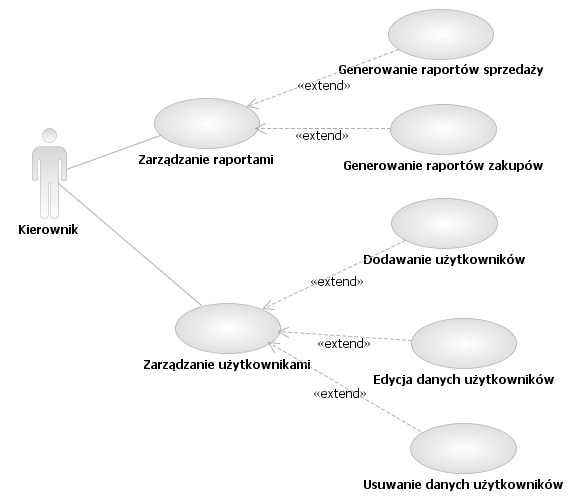
\includegraphics[angle=-90,scale=0.8]{../img/kierownikUseCase.png}
    \end{center}
    \label{fig:kierownikUseCase}
\end{figure}

\begin{figure}[h]
    \begin{center}
    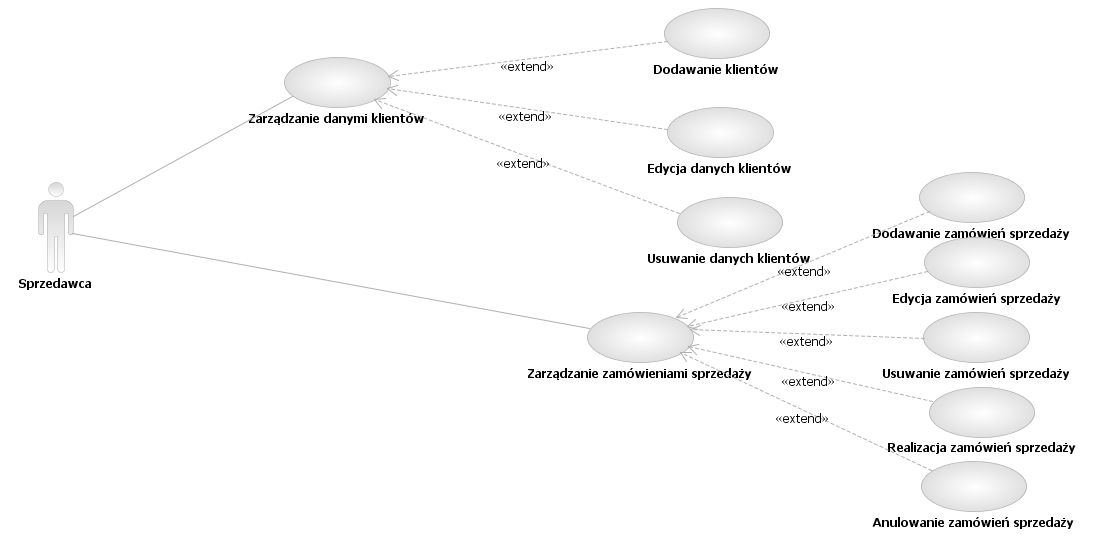
\includegraphics[angle=-90,scale=0.75]{../img/sprzedawcaUseCase.png}
    \end{center}
    \label{fig:sprzedawcaUseCase}
\end{figure}

\begin{figure}[h]
    \begin{center}
    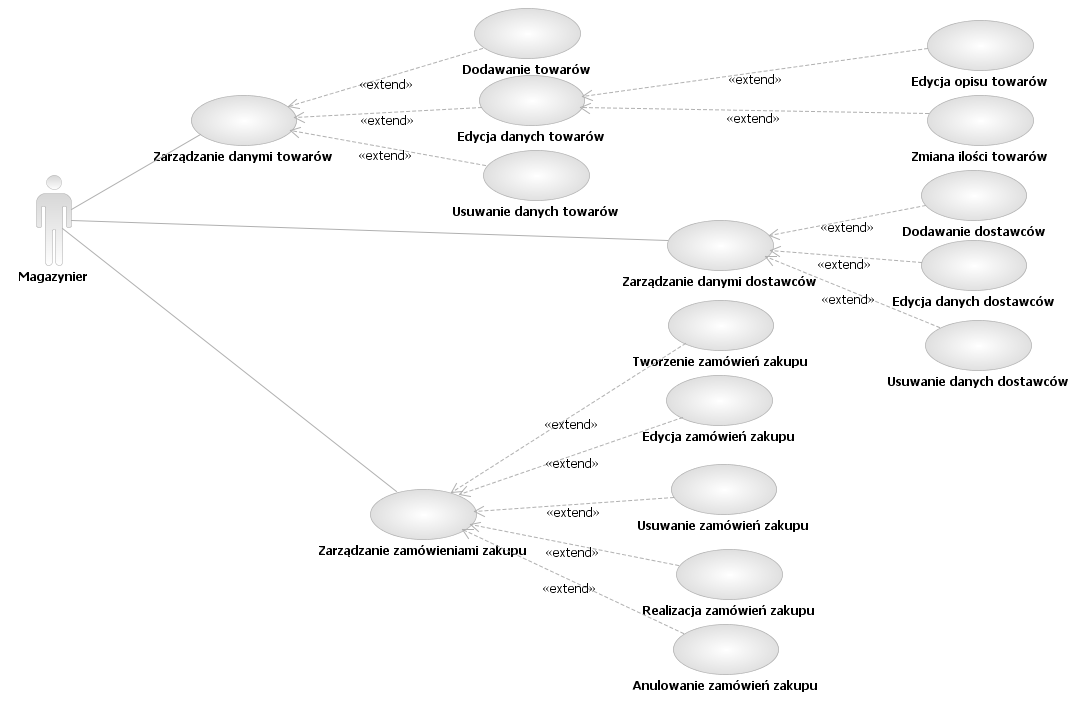
\includegraphics[angle=-90,scale=0.75]{../img/magazynierUseCase.png}
    \end{center}
    \label{fig:magazynierUseCase}
\end{figure}